% Capítulo: Design and Implementation
% Codificación: UTF-8

\chapter{Design and Implementation}
\label{chap:design}

The main objective of this thesis is to develop an executable specification
of PISA using ASL. The specification must be a definition of the instruction set that
can be read as its documentation and run as its reference. Specifying the
whole of PISA is beyond the scope of a thesis, so the specification covers
a subset, chosen so that the part of PISA that is distinctive of GPU
execution, the divergence and reconvergence of a sub-group, is given a
complete model of its own. This chapter presents the specification and the system built around
it to make it run.

The system has three components, shown in Figure~\ref{fig:system-overview}.
The specification, written in ASL, defines the architectural state of a
PISA sub-group and the semantics of each instruction of the subset, and
executes a kernel step by step over that state. Because PISA exists only as
text, with no binary encoding for the specification to decode, a parser
translates a PISA kernel into the ASL code that sets up the kernel's state
and instruction stream. The specification and the generated code are
compiled to C, and a host library wraps the result in an OpenCL-style
interface, so that a host program allocates buffers, launches kernels, and
reads results from the specification as it would from any OpenCL device.

\begin{figure}[t]
  \centering
  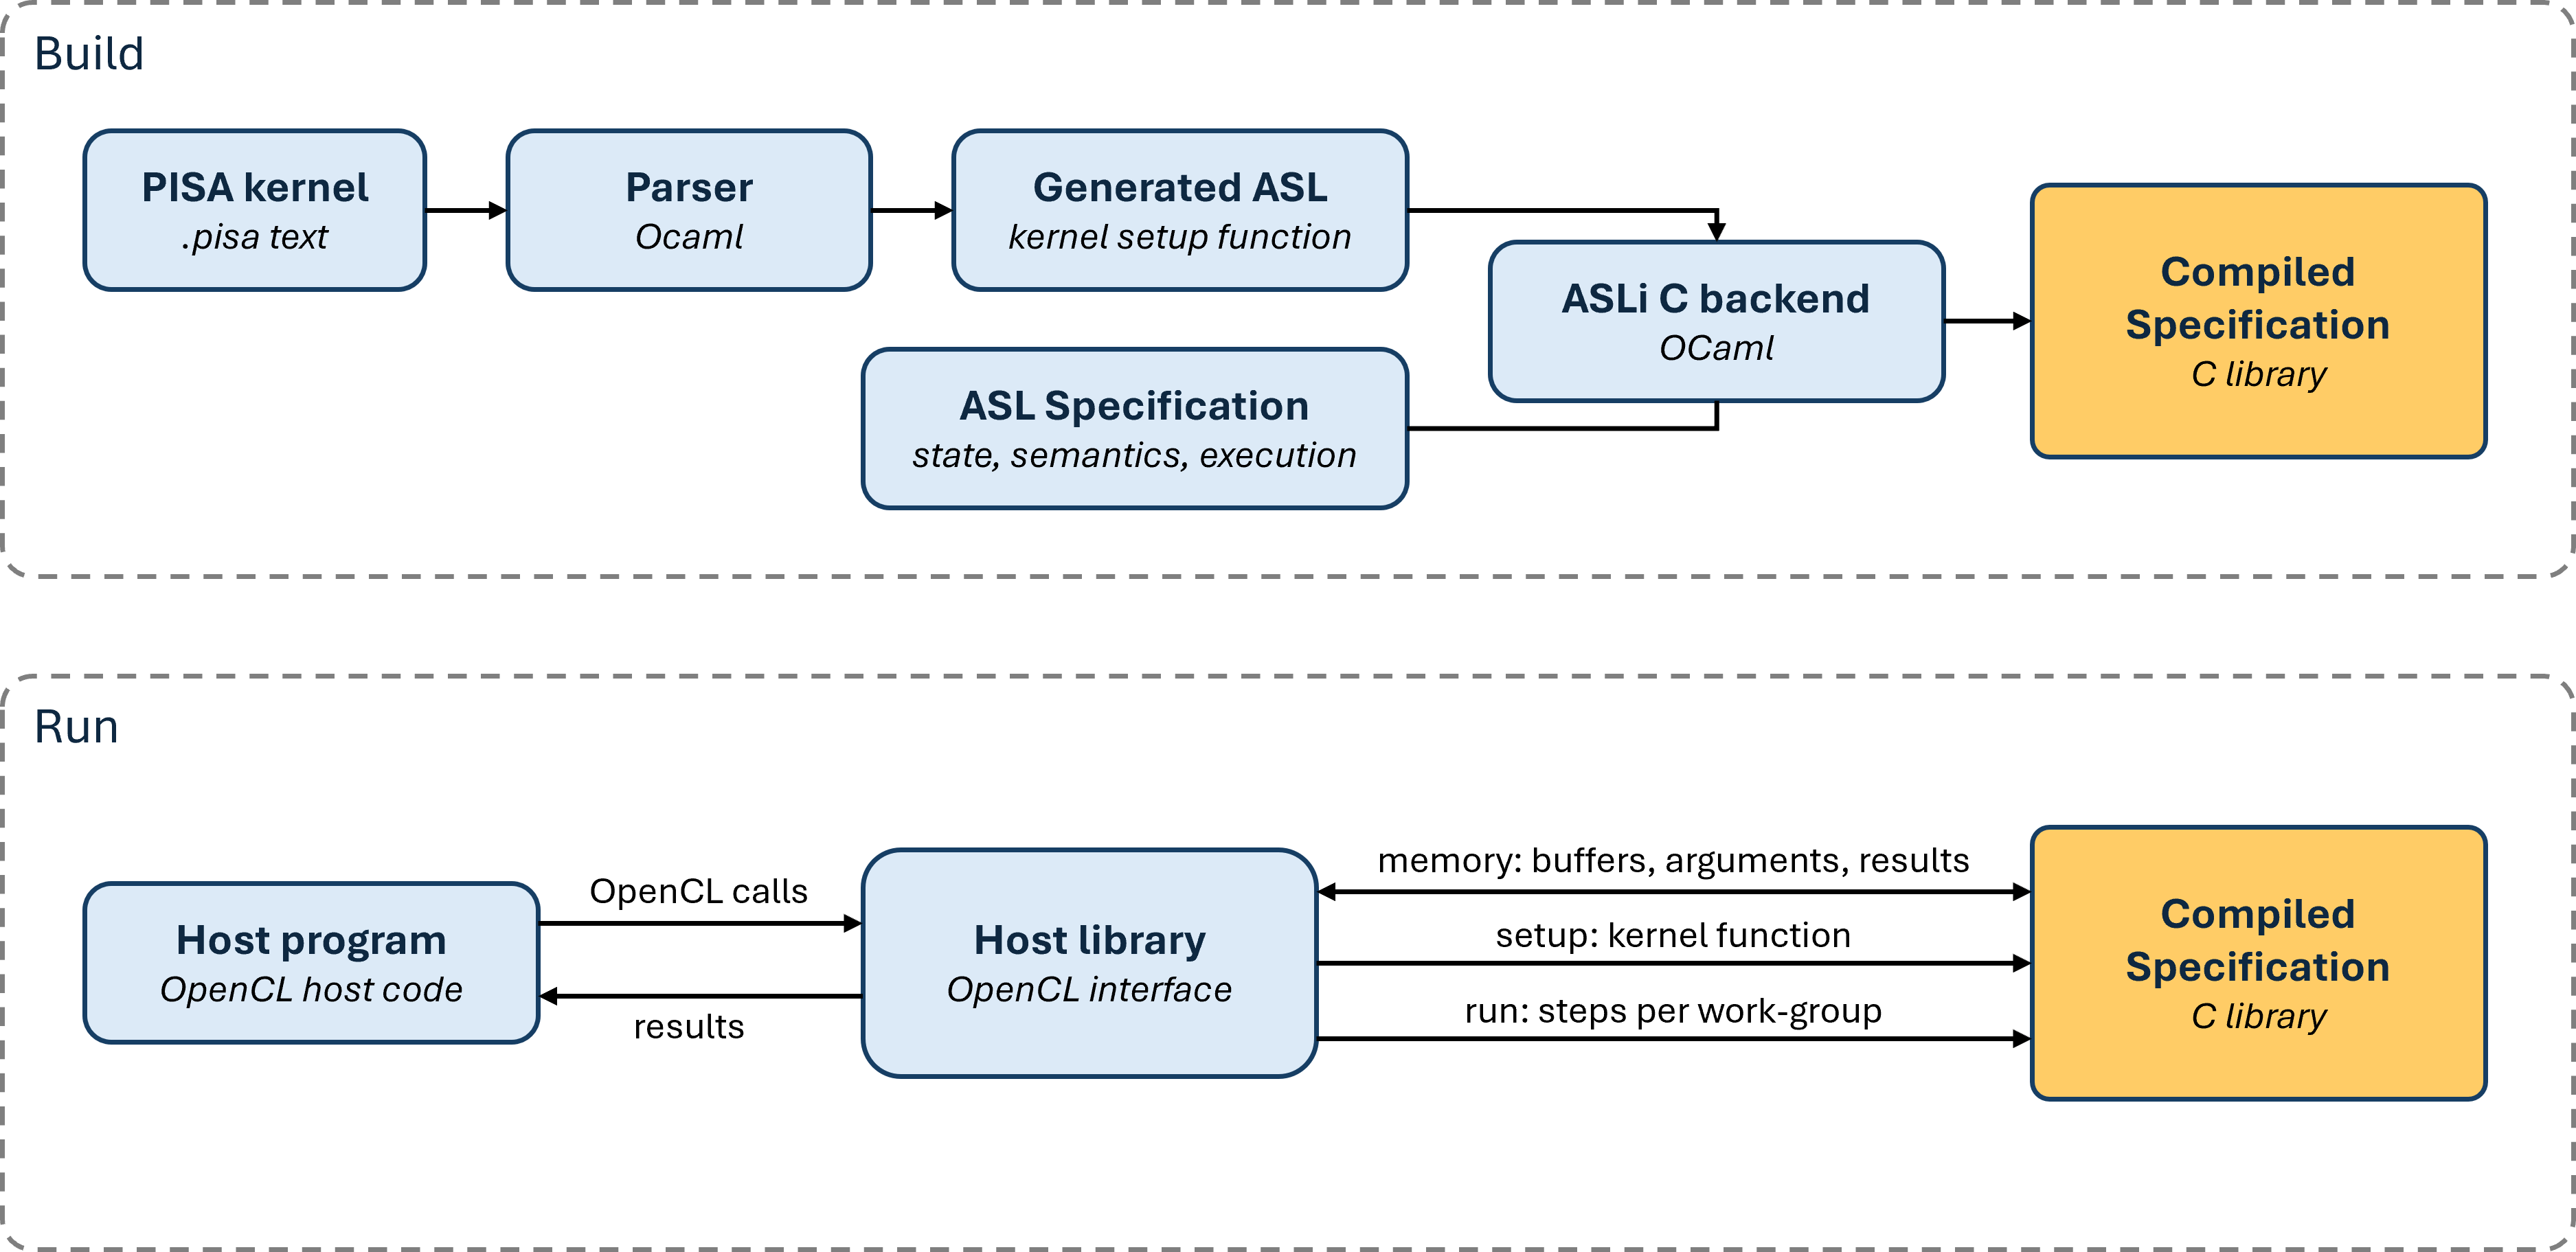
\includegraphics[width=\textwidth]{img/spec-overview.png}
  \caption[Architecture of the specification]{Architecture of the
  specification. Above, a PISA kernel is parsed into an ASL setup
  function and compiled, together with the specification, into a C
  library. Below, a host program drives that library through the OpenCL
  interface of the host library.}
  \label{fig:system-overview}
\end{figure}

The chapter follows this structure. Section~\ref{sec:pisa-subset} defines
the subset of PISA that is specified: what it contains, what it leaves out,
and the execution model it adopts. Section~\ref{sec:asl-spec} presents the
ASL specification itself: its state, its instruction semantics, the
execution model, and the handling of divergence. Section~\ref{sec:parser}
describes the parser, and Section~\ref{sec:host-library} the host library.


%--------------------------------------------------%
\section{The PISA Subset}
\label{sec:pisa-subset}

The specification covers a subset of PISA, selected so that the execution
of a sub-group can be specified completely. Throughout this document,
\emph{the subset} refers to the part of PISA defined in this section.
Within it, instruction semantics follow the published PISA specification
without modification~\cite{pisa-spec}.

Table~\ref{tab:subset-instructions} lists the instructions of the subset
by class. Every
instruction listed is supported in all of its variants.
The subset contains the instructions a kernel needs to read its inputs
from the host and write its results back, the control flow with which a
sub-group diverges and reconverges, and the instructions through which
the work-items of a sub-group communicate. It is complete enough to run
real workloads compiled from OpenCL.

\begin{table}[t]
\centering
\begin{tabular}{ll}
\toprule
Class & Instructions \\
\midrule
Logic and shift          & \texttt{and}, \texttt{or}, \texttt{xor}, \texttt{shl}, \texttt{shr}, \texttt{asr} \\
Comparison and selection & \texttt{scmp}, \texttt{ucmp}, \texttt{sel} \\
Control flow             & \texttt{goto}, \texttt{return} \\
Integer arithmetic       & \texttt{iadd}, \texttt{isub}, \texttt{smul}, \texttt{sdiv}, \texttt{udiv}, \texttt{smad}, \texttt{umad} \\
Memory                   & \texttt{ld}, \texttt{st} \\
Movement and conversion  & \texttt{mov}, \texttt{sext}, \texttt{zext}, \texttt{trunc} \\
Sub-group communication  & \texttt{shfl}, \texttt{ired} \\
\bottomrule
\end{tabular}
\caption{Instructions of the subset.}
\label{tab:subset-instructions}
\end{table}

Some major functionalities of PISA were left out of the subset to keep the
work within scope, and each omission has a cost on what the subset can do.
Floating point instructions were left out, since implementing them means
implementing the floating point logic under the IEEE rules. The cost is
that the subset cannot support any floating point workload. However, integer
arithmetic is sufficient for what this thesis wants to achieve. Function
calls were left out as well, since the specification would have to keep a call
stack per lane and reconverge lanes across calls. The cost is that the
specification cannot run a kernel whose functions a
compiler does not inline. Synchronization instructions, such as barriers, fences and atomics, were also
left out, since the specification would have to run the sub-groups of a
work-group side by side and define how they wait for one another and in
what order their memory accesses become visible. The cost is that the
specification guarantees no order of memory accesses or of instruction
execution across sub-groups, so a workload in which work-groups or
sub-groups exchange data can be racy. The remaining instructions of PISA
were left out for lack of time, or because they are newer than the
implementation of the specification. Their absence however, does not affect the
behavior of the specification. None of this is because of a limit of the specification itself,
and each omission can be added in future work.

The execution model of the subset is restricted to execution within a
sub-group. A work-group consists of one or more sub-groups of 32
work-items, so its size is a multiple of 32. A host program performs one
kernel launch, over an NDRange of such work-groups, and the model executes
the work-groups, and the sub-groups of each, one after another. Each
sub-group begins with its launch context set from the launch parameters,
which are accessible through the special registers. PISA does not define
how the work-items of a sub-group execute relative to one another. The
subset adopts lockstep execution: at each step, the active work-items
execute one instruction.


\section{The ASL Specification}
\label{sec:asl-spec}

The ASL specification is an executable model of the subset. It represents
the architectural state of one sub-group and defines, for each
instruction, how that state is transformed. A kernel runs by repeatedly
selecting the next instruction and applying its semantics to the state,
until every work-item of the sub-group has terminated.

PISA, being a virtual ISA, leaves parts of its execution open, to be
defined by each implementation that adopts it. This specification, being
an executable model, must define them as well. These definitions are
choices of the specification and are marked as such where they are made.

Section~\ref{sec:asl-state} describes the state of the model.
Section~\ref{sec:asl-instructions} describes how instruction semantics are
encoded as ASL functions. Section~\ref{sec:asl-execution} describes how
the specification executes one instruction across the sub-group, and
Section~\ref{sec:asl-divergence} how it selects the next.

\subsection{State Model}
\label{sec:asl-state}

The state of the specification is everything a sub-group's execution can
observe or modify. It falls into three groups: the memory regions that
model PISA's address spaces, the instruction buffer that holds the
program, and the execution state of each lane and of the sub-group as a
whole. Listing~\ref{lst:state-decls} shows the global declarations that
constitute it, in that order.

\begin{lstlisting}[caption={The specification's state declarations.}, label={lst:state-decls}]
// Memory: one region per address space
var RegisterSpace  : __RAM(32);
var PrivateSpace   : __RAM(32);
var SharedSpace    : __RAM(32);
var ConstantSpace  : __RAM(64);
var GlobalSpace    : __RAM(64);
var ParameterSpace : __RAM(64);

// Program
var MaxPC = 1024;
var InstructionBuffer : array[MaxPC] of Instruction;

// Execution state
var PC         : array[32] of integer;
var Done       : bits(32);
var GlobalPC   : integer;
var ActiveMask : bits(32);
\end{lstlisting}

\paragraph{Memory regions.} Each of PISA's six address spaces is a
separate \lstinline{__RAM} region, declared with an address width per
space: 32 bits for the register, private, and shared spaces, 64 bits for
the constant, global, and parameter spaces.
Separate regions apply PISA's rule that an address is interpreted within
its space: the same numeric address in two regions names two different
locations, and an instruction reaches only the region its space qualifier
names. A region has no fixed size, \lstinline{__RAM} provides the whole
address range of its width, and an address that has not been written
reads as zero.

\paragraph{Per-lane layout.} The register and private regions hold
per-work-item storage: every lane has its own copy of each register and
each private variable. A variable in these regions is therefore laid out
as 32 consecutive elements, one per lane, and a lane reaches its
element by offsetting the variable's base address by its lane index.
Figure~\ref{fig:lane-layout} shows the layout against that of a shared
variable, which exists once and is reached by every lane at the same
address. The constant, global, and parameter regions share the same layout.
Predicate registers follow the per-lane layout with one-bit elements.
Special registers are allocated in the register region and written at
kernel setup.  Some of those values can change during
execution, such as the active mask. For those their value is computed from the
execution state when read.

\begin{figure}[htbp]
    \centering
    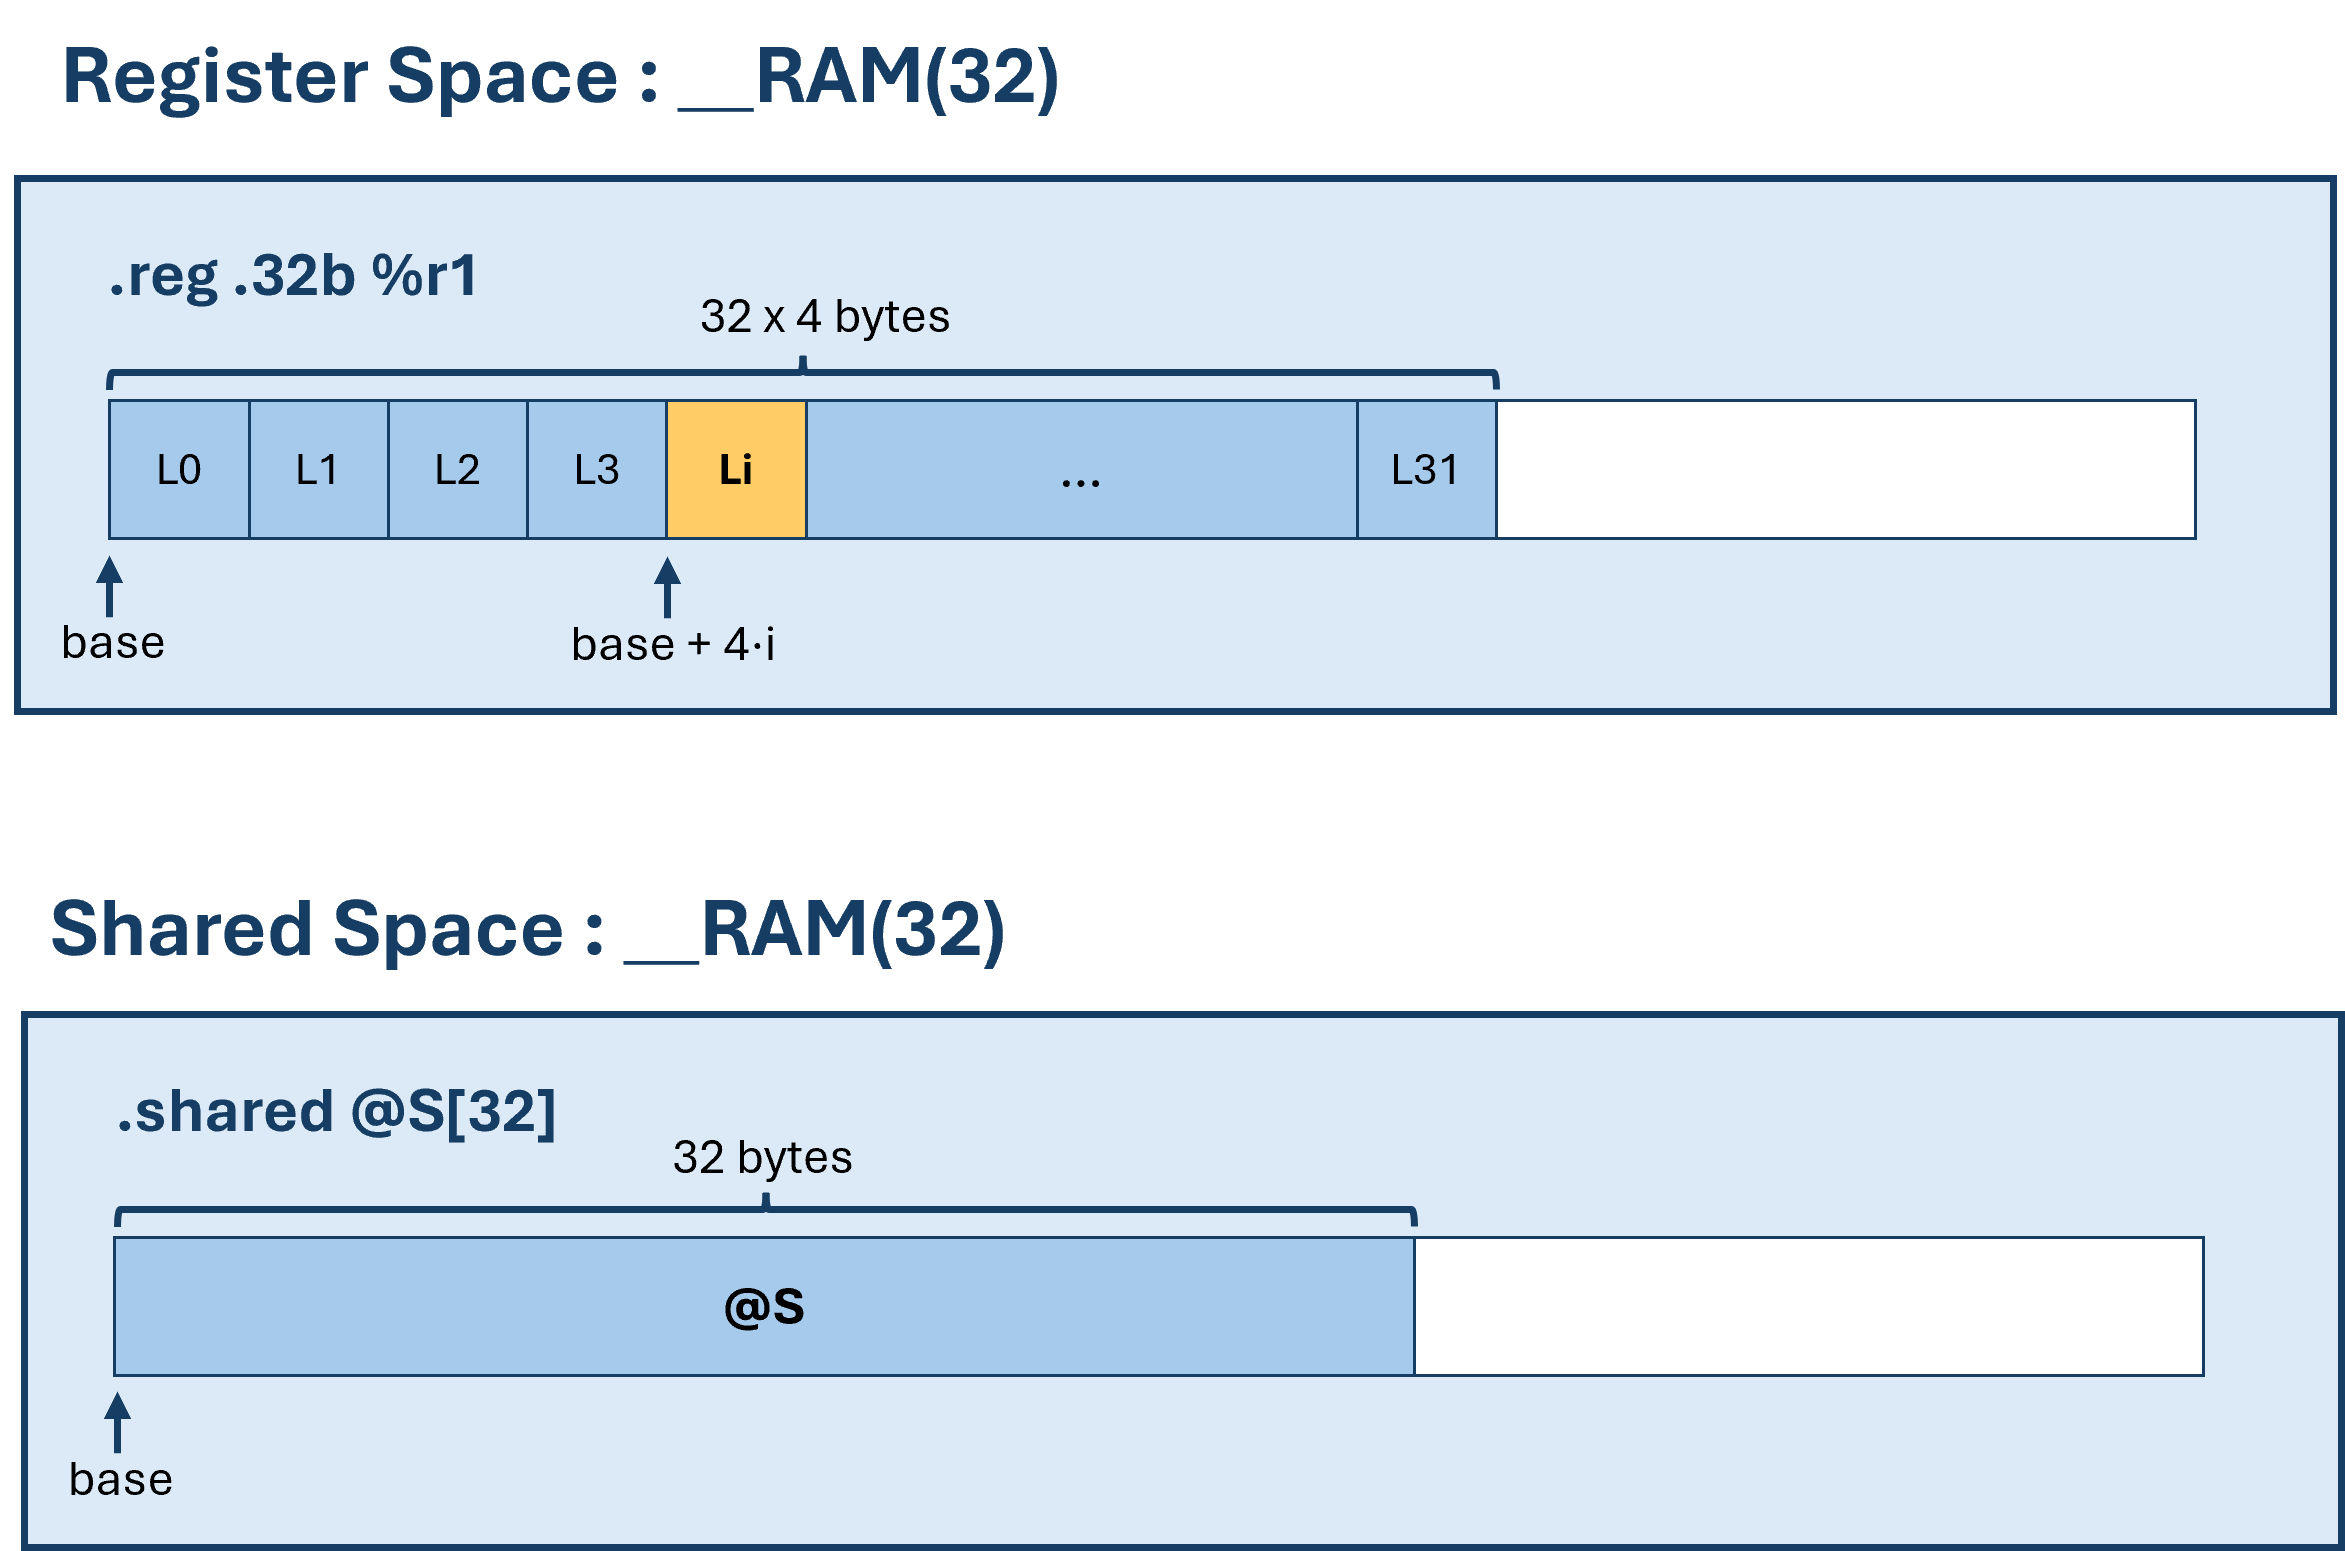
\includegraphics[width=0.85\textwidth]{img/memasl.png}
    \caption[Per-lane layout]{A register variable and a shared variable in their regions.}
    \label{fig:lane-layout}
\end{figure}

\paragraph{The variable map.} A kernel declares its variables by name, but the specification stores
them at addresses inside the memory regions, so a variable map is needed
to link the two. For every declared variable it records which region the
variable was placed in and at what address, so that an instruction that 
uses the variable as an operand can access it. It is an array of records,
Listing~\ref{lst:variable-record}, one per declared variable, holding the
variable's name, the space it lives in, its base address in that space,
its total size, and its per-lane stride. The map is also where storage is
allocated: when the setup code of a kernel declares a variable, the
specification computes its size in bytes, places it at the next free
address of its space, records the entry, and advances that space's free
pointer. The bases of Figure~\ref{fig:lane-layout} are assigned here. A
variable is identified by an integer id, assigned by the parser
(Section~\ref{sec:parser}), the emitted instructions refer to variables by
id, and the specification resolves an id to its record by searching the
array.

\begin{lstlisting}[caption={A variable-map entry.}, label={lst:variable-record}]
record Variable {
    id      : integer;        // id assigned by the parser
    name    : string;
    space   : AddressSpace;   // __RAM region
    address : bits(64);       // base address in that region
    size    : integer;        // total size in bytes
    offset  : integer;        // per-lane stride
}

var Variables : array[128] of Variable;
\end{lstlisting}


\paragraph{The program.} The kernel is held in an instruction buffer, an
array of size \lstinline{MaxPC} with one record per instruction. Listing~\ref{lst:instruction-record}
shows the record: it is wide enough to describe any instruction of the
subset, with a field for each piece of information some instruction
needs, from the opcode and operand width to the operands, immediates,
address operands, branch target, and qualifiers. Operands are represented as their ids in the
variable map, so to resolve an operand it needs to be looked up by id. The buffer is
filled by the setup code the parser generates (Section~\ref{sec:parser}),
one record per instruction of the kernel, in program order. Positions in
the buffer are the program counter values used throughout execution: a
program counter is an index into the buffer, and advancing a lane past an
instruction increments its index. Labels occupy positions of their own, as records whose opcode marks them
as labels, so a label is a program counter value like any other.

\begin{lstlisting}[caption={The instruction record (excerpt). An instruction buffer entry carries every field any instruction of the subset may need. The fields not used by an instruction are left unset.}, label={lst:instruction-record}]
record Instruction {
    opcode    : Opcode;
    bitwidth  : integer {8, 16, 32, 64};

    // operands, as variable ids
    dst       : integer;
    src0      : integer;
    src1      : integer;
    src2      : integer;
    src3      : integer;

    // immediates: flag and value per source position
    use_imm0  : boolean;
    use_imm1  : boolean;
    use_imm2  : boolean;
    use_imm3  : boolean;
    imm0      : integer;
    imm1      : integer;
    imm2      : integer;
    imm3      : integer;

    // memory access
    write_addr : boolean;
    read_addr  : boolean;
    dst_addr   : AddressOperand;
    src_addr   : AddressOperand;

    // label identifier
    label     : integer;

    // pretty print of the instruction in PISA format
    debug_string : string;

    // qualifiers
    ci        : bit;
    co        : bit;
    precision : bit;
    addrspace : AddressSpace;
    ...
}

var InstructionBuffer : array[MaxPC] of Instruction;
\end{lstlisting}

\paragraph{Execution state.} Each lane has a program counter, its
position in the instruction buffer, and a termination flag, set when the
lane executes a \texttt{return}. Because each lane has its own counter,
lanes may stand at different positions in the program, which is what
makes divergence representable. The sub-group has a global program
counter, the position of the instruction being executed in the current
step, and an active mask, one bit per lane, marking the lanes that execute
it. The \texttt{\%activemask} special
register returns this value. These values change as the kernel executes: the per-lane counters through
the control-flow instructions, and the global counter and the mask through
the specification's reconvergence mechanism.

\subsection{Instruction Semantics}
\label{sec:asl-instructions}

The semantics of each instruction of the subset are defined by an ASL
function. These functions are the executable counterpart of the
instruction's documentation in PISA: each
is the pseudocode that describes what the instruction computes, and
also the code that runs to produce that
effect. Conceptually an instruction operates on the sub-group as a whole,
one instruction applied at once across all participating lanes. Each semantic
function, however, defines the operation for one lane, and
the specification's execution model applies it across the active lanes.

For most instructions the semantic function is pure. It receives the
operand width, the instruction record, and the raw values of the source
operands, and returns the raw result, without touching the
specification's state. The reads that supply the source values and the
write that stores the result are performed by the execution model, not by
the function. A minority of instructions access state directly within
their functions: loads, branches, and the sub-group
communication instructions, since reading a memory region,
redirecting control flow, or exchanging values across lanes is the
instruction's essential effect. Keeping state accesses out of the common
case leaves each semantic function focused on the operation itself, so
that the pseudocode a reader sees expresses the instruction's behavior
without the surrounding load and store machinery, in the style of an
architecture manual. It also makes each function callable on its own,
with operands supplied directly.

Operand-width polymorphism is handled by passing the width as a
parameter. A single function serves every width variant of an instruction
by operating on the relevant slice of its operands and producing a result
of the corresponding width. Listing~\ref{lst:and_asl_impl} shows the
semantic function for the bitwise \texttt{and} instruction.

\begin{lstlisting}[caption={The semantic function of the bitwise \texttt{and} instruction. Annotated.}, label={lst:and_asl_impl}]
func and(bitwidth : integer {16, 32, 64},
         instruction : Instruction,
         src0 : bits(64),
         src1 : bits(64)) => bits(64)
begin
    var result : bits(64) = Zeros(64);

    // Extract operands at specified bit width
    let operand0 = src0[0 +: bitwidth];
    let operand1 = src1[0 +: bitwidth];

    // Perform bitwise AND operation
    let and_result = operand0 AND operand1;

    // Package result in standardized container
    result[0 +: bitwidth] = and_result;

    return result;
end
\end{lstlisting}

The function admits widths of 16, 32, or 64 bits. The source operands
arrive as 64-bit containers, of which the low \texttt{bitwidth} bits are
significant. The function extracts the operands at the requested width,
computes the result, and returns it in a container of the same form. The
instruction record is available for instructions whose behavior depends on further fields, such as a
comparison relation or a shuffle pattern. The
result is written to the instruction's destination by the execution
model.

\subsection{SIMT Execution Model}
\label{sec:asl-execution}

Execution of a kernel proceeds as a sequence of steps. At each step, the
sub-group executes the single instruction at the global program counter, on
behalf of the lanes that are currently active, and then advances. Execution
continues until every lane has terminated. This is the lockstep execution
adopted in Section~\ref{sec:pisa-subset}: at each step, one instruction is
applied across the active lanes. The specification executes each step
sequentially, visiting the active lanes one at a time, and the result is
equivalent to simultaneous execution because every read of the step happens
before any of its writes.

Every instruction that produces a value runs through a common two-pass
scheme, shown in Figure~\ref{fig:execution-step}. In the first pass, the
execution model visits each active lane in turn. For the lane, it reads
the source operands (registers at the lane's offset, special registers
from the execution state, immediates from the instruction record,
effective addresses from base and offset), calls the semantic function
selected by the opcode, and holds the result. In the second pass, it
visits the active lanes again in the same order and writes the held
results to their destinations, a register or a memory location. Because
no write happens until every lane has read, each lane's function sees the
state as it stood at the start of the step, whatever the order in which
lanes are visited. This matters when one lane's source is another lane's
destination, as in a shuffle or a reduction. \texttt{shfl} runs in the
common scheme and differs from other instructions only in reading its
source value from the selected lane's register rather than the issuing
lane's. \texttt{ired} does the same for all the active lanes at once: each
lane's function reads the contributions of every active lane and computes
the aggregate, and each lane holds and then writes its own copy. Since
the second pass writes in lane order, when several lanes write the same
memory location in one step, the value of the last lane remains.

\begin{figure}[t]
  \centering
  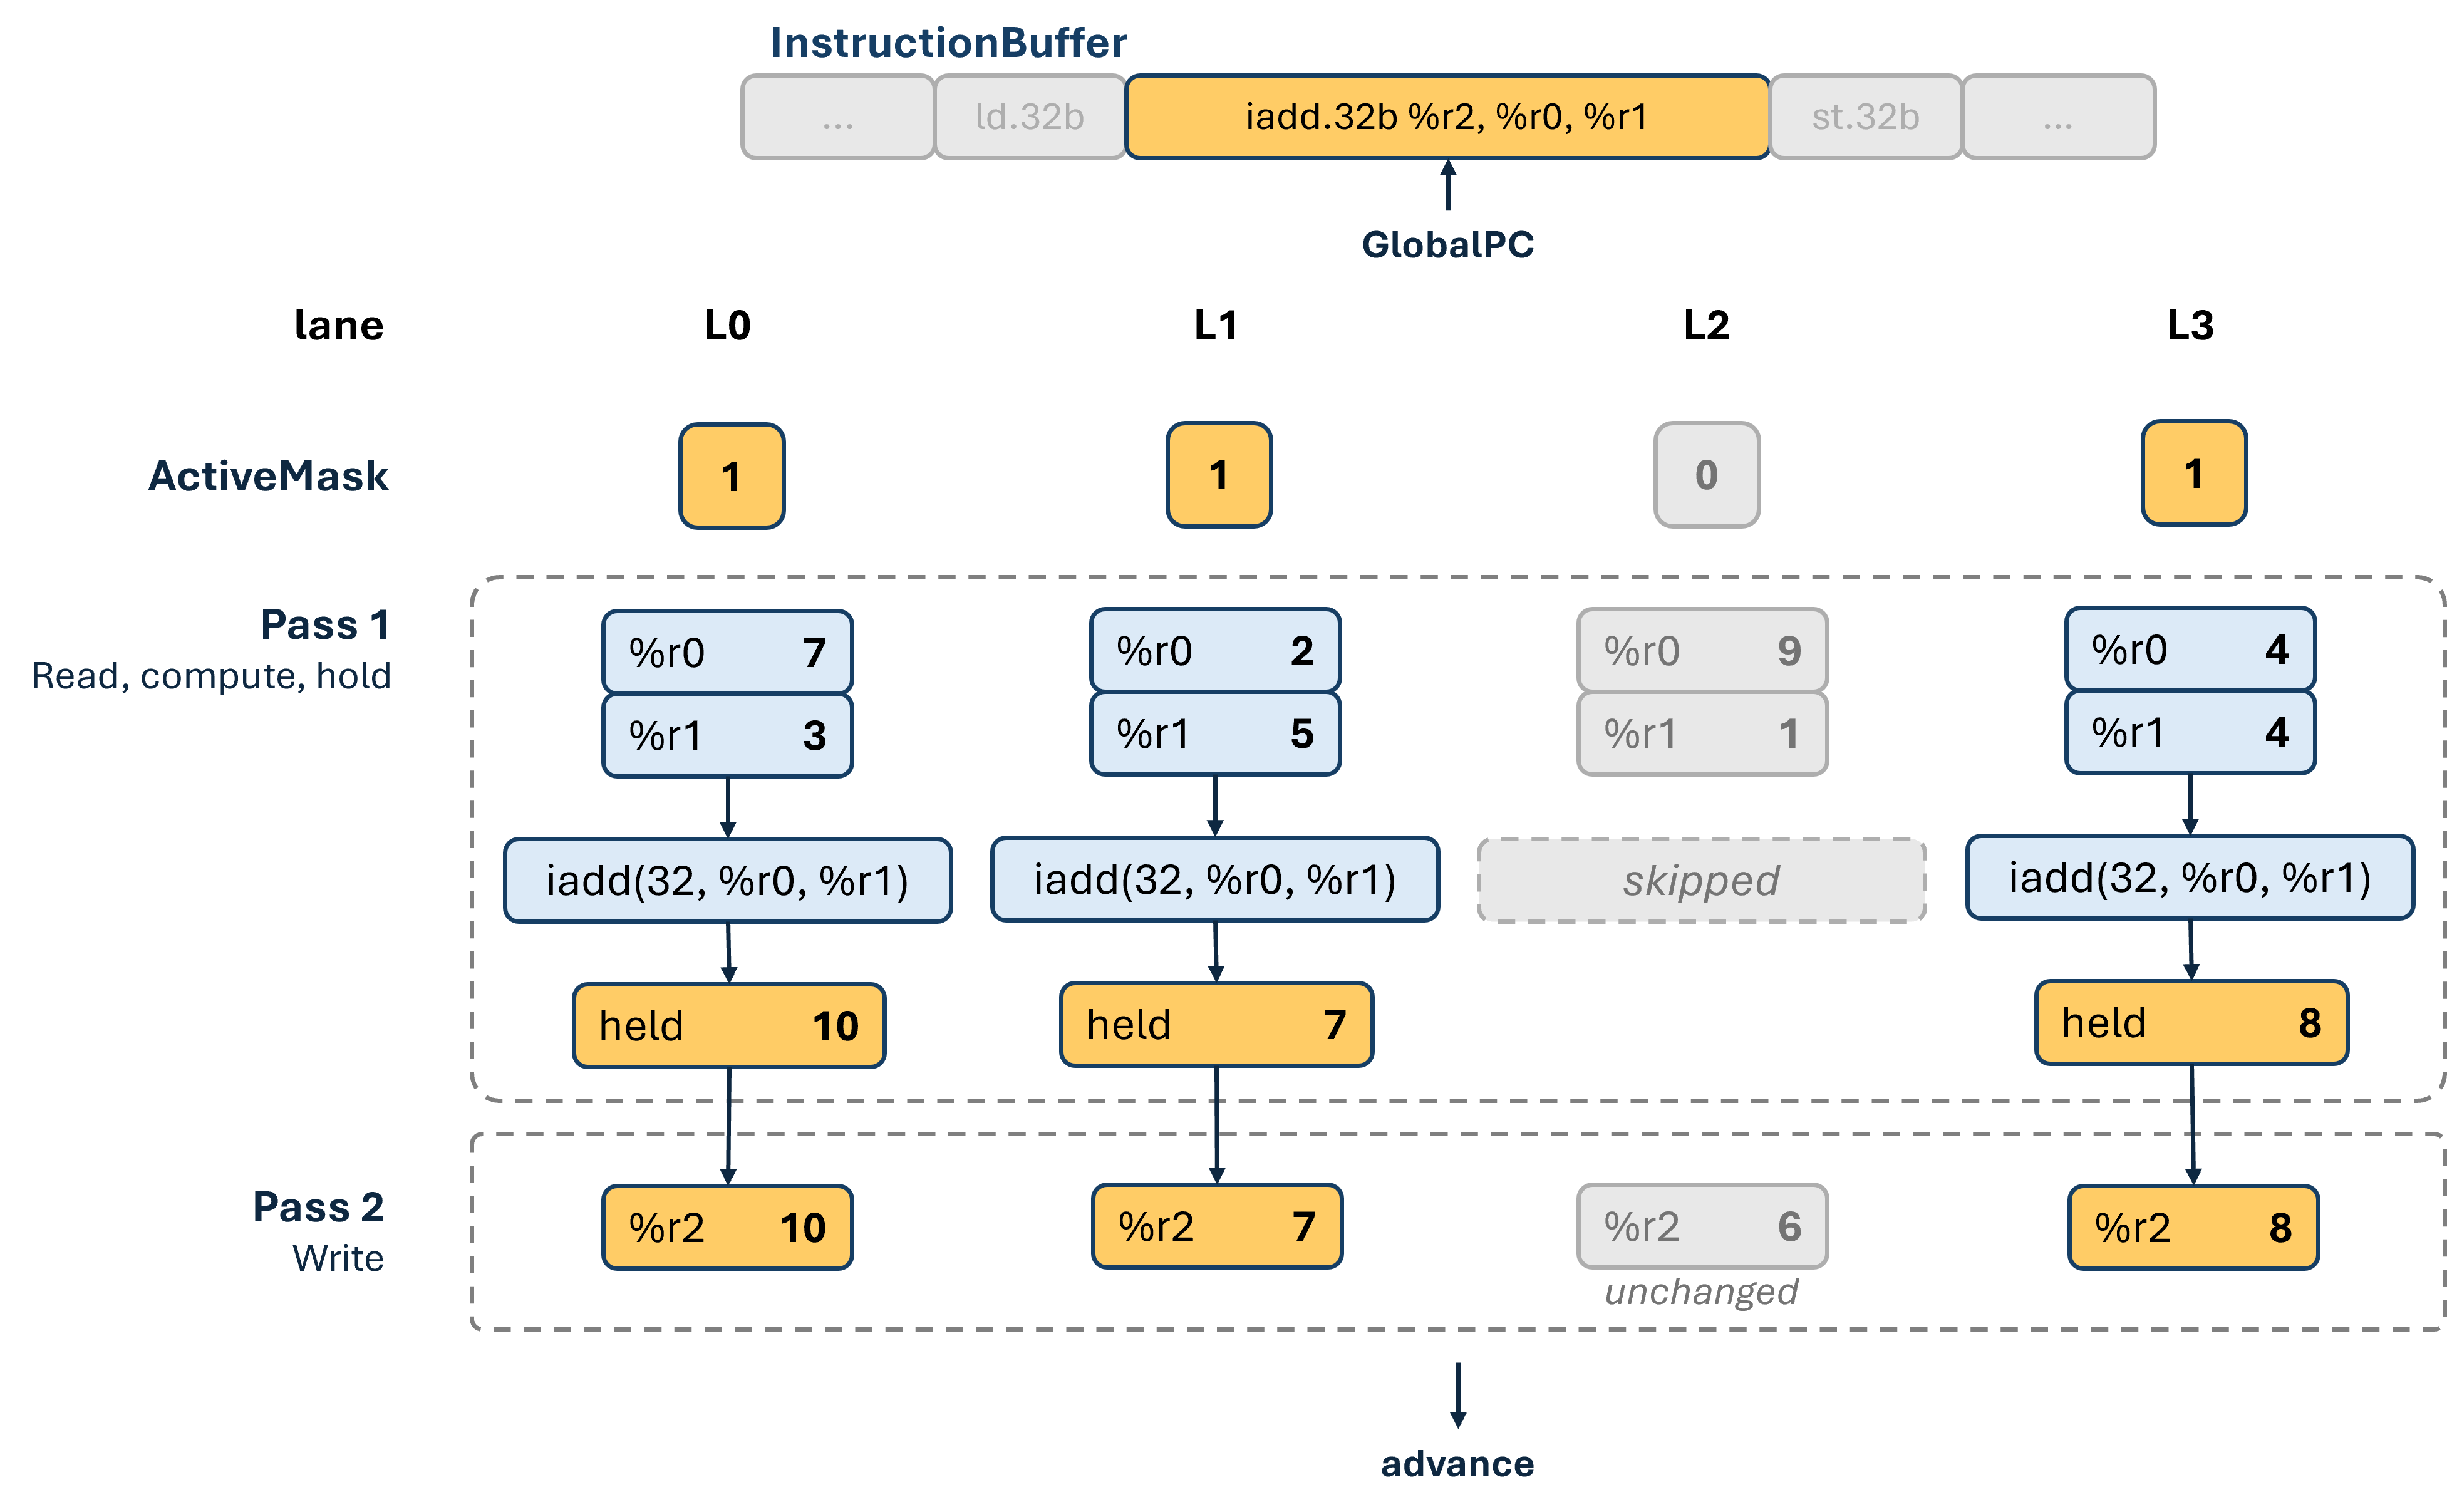
\includegraphics[width=\textwidth]{img/execution-step.png}
  \caption[One execution step]{One execution step of the common scheme.
  The instruction at the global program counter is applied to the active
  lanes: the first pass reads each lane's operands and holds the result,
  and the second pass writes the held results back. Lane 2 is inactive
  and is skipped, so its registers are unchanged.}
  \label{fig:execution-step}
\end{figure}

The \texttt{return} and \texttt{goto} instructions are the exception. They write to no
destination and only change the execution state, so they apply their
effect in the first pass: a return sets the lane's termination flag and
deactivates the lane, and a branch sets the lane's program counter. The
state they change is consulted between steps, so neither disturbs the
separation of reads and writes.

After an instruction has been executed for all active lanes, the
sub-group advances to the next step. Without divergence, every active
lane's program counter moves to the following instruction and the global
program counter advances with it. With divergence, the active lanes and
the global program counter of the next step depend on which branches the
lanes took.

\subsection{Divergence and Reconvergence}
\label{sec:asl-divergence}

The most complicated part of the execution model is its handling of
divergence. When the active lanes execute a conditional branch, they may not
all take the same direction: some will jump to the target while others fall
through, so the lanes will no longer share the same position in the program. 
Lockstep execution applies one instruction per step to all the active
lanes, so after a divergent branch, when the lanes point at different
instructions, the specification must decide which of them to run and which
will wait, and when the waiting lanes rejoin. It
must do so without reconvergence markers in the instruction stream, since
PISA exposes control flow purely as branches.

PISA defines no reconvergence mechanism, so the
specification must choose one. It resolves divergence with the implicit stackless
scheme described by Collange~\cite{collange-stackless}, which needs no
reconvergence stack and no explicit join points. This mechanism rests only on the
per-lane program counters. At the start of each step,
the global program counter is set to the minimum of the program counters
over the lanes that have not terminated, and then each lane whose counter
equals to that minimum is reactivated (Listing~\ref{lst:min-pc}). 
The instruction at the global program counter is then executed for the
active lanes. Afterwards, each active lane's counter is updated to the
next instruction, or, for a taken branch, to its target.

\begin{lstlisting}[caption={The scheduling rule, run at the start of each
step.}, label={lst:min-pc}]
func SetMinPC()
begin
    var minPC = MaxPC;
    for lane = 0 to 31 do
        if (Done[lane] == '0') && (PC[lane] < minPC) then
            minPC = PC[lane];
        end
    end
    GlobalPC = minPC;
end

func Reconverge()
begin
    for lane = 0 to 31 do
        if (Done[lane] == '0') && (ActiveMask[lane] == '0') && (PC[lane] == GlobalPC) then
            ActiveMask[lane] = '1';
        end
    end
end
\end{lstlisting}

The branch instruction does the other half of the work
(Listing~\ref{lst:goto}). A lane that executes a conditional branch sets its program
counter to the target if the predicate holds, and to the next instruction otherwise. 
For the unconditional case the branch always takes the target. The lane then marks 
itself inactive. The branch does not know whether the sub-group diverged, and it does not decide which
lanes continue: that is left to the scheduling rule at the start of the next
step. If every lane took the same direction, the rule activates them all
again and execution continues as before. If they split, the rule activates
the lanes with the lower counter and leaves the others waiting, inactive,
with their counters untouched. At each step it runs whichever lanes are
furthest behind, and when the counters coincide the lanes are active
together again. Together, the branch and the rule guarantee that, at the start of every
step, the active lanes are exactly the non-terminated lanes at the lowest
counter. Divergence and reconvergence follow from this guarantee, with no
reconvergence point recorded anywhere. The per-lane counters do the work a
reconvergence stack does in conventional implementations.

\begin{lstlisting}[caption={The semantic function of \texttt{goto}.},
label={lst:goto}]
func goto(lane : integer, pred : bit, instruction : Instruction)
begin
    let cond = instruction.goto_cond;
    let label_pc = GetLabelPC(instruction.label);
    var predicate : bit;

    if cond then
        predicate = pred;

        if instruction.flip then
            predicate = NOT predicate;
        end

        if predicate == '1' then
            PC[lane] = label_pc;
        else
            PC[lane] = GlobalPC + 1;
        end
    else
        PC[lane] = label_pc;
    end
    ActiveMask[lane] = '0';
end
\end{lstlisting}

The specification assumes that the last instruction of a kernel is a
\texttt{return}. Under this assumption no counter ever points outside the
instruction buffer: a counter moves only to
a branch target, which the parser has resolved to a slot of the buffer, or
to the next instruction, which exists for every instruction but the last,
and a lane that reaches the last instruction terminates. For a lane that
reads no value produced by another lane, execution is exactly the
sequential execution of its path: the lane runs only at its own counter,
its registers are its own, and each of its writes is complete before its
next step. Where lanes communicate, this no longer holds. A shuffle, a reduction or a
read of the mask register gives a result that depends on which lanes are
active at that step, and a value passed through memory depends on which
lane wrote it last. Both depend on the schedule.

Diverged lanes rejoin where the two paths of a branch meet again, provided
that meeting point comes after both paths in the instruction order, as it
usually does in compiler-emitted code~\cite{collange-stackless}. In other
layouts the lanes rejoin later, or elsewhere, which does not change the
results of lanes that do not communicate. A waiting lane can be starved
only by a lane behind it that never terminates. The specification places
no bound on the number of steps, so such a kernel does not complete.

Table~\ref{tab:divergence-if-else} traces the execution of a kernel with
an \texttt{if}-\texttt{else} region, over a sub-group of four lanes rather
than 32, for readability. Label slots are omitted here and in
Table~\ref{tab:divergence-loop}. The program computes a predicate that is
true for lanes~0 and~1 and false for lanes~2 and~3, branches to the
\texttt{else} block when the predicate is false, executes the
\texttt{then} block at instruction~2, branches past the \texttt{else}
block at instruction~3, executes the \texttt{else} block at
instruction~4, and reconverges at instruction~5. After the branch at
step~2, lanes~0 and~1 take the \texttt{then} path while lanes~2 and~3
wait at the \texttt{else} block. Once the \texttt{then} lanes branch past
it to instruction~5, the scheduling rule selects the waiting lanes, which
execute the \texttt{else} block and rejoin the others at step~6.

\begin{table}[h]
\centering
\begin{tabular}{c c c c l}
\toprule
Step & PCs [L0\,L1\,L2\,L3] & Global PC & Active mask & Instruction \\
\midrule
1 & 0\;0\;0\;0 & 0 & 1111 & compute predicate \\
2 & 1\;1\;1\;1 & 1 & 1111 & branch if not predicate $\to$ 4 \\
3 & 2\;2\;4\;4 & 2 & 1100 & then block \\
4 & 3\;3\;4\;4 & 3 & 1100 & branch $\to$ 5 \\
5 & 5\;5\;4\;4 & 4 & 0011 & else block \\
6 & 5\;5\;5\;5 & 5 & 1111 & end (reconverged) \\
\bottomrule
\end{tabular}
\caption{Execution trace of an \texttt{if}-\texttt{else} region.}
\label{tab:divergence-if-else}
\end{table}

Table~\ref{tab:divergence-loop} traces a loop in which lanes iterate a
different number of times: lanes~0 and~1 perform one iteration, and
lanes~2 and~3 perform two. The loop tests its condition at instruction~1,
branches out to instruction~5 when the condition fails, and returns to
the test with a backward branch at instruction~4. At step~7 the condition
fails for lanes~0 and~1, which branch to the exit and wait there. Lanes~2
and~3 remain at lower program counters and continue looping, in steps~8
to~11, until they too reach the exit, and all four lanes rejoin at
step~12.

\begin{table}[h]
\centering
\begin{tabular}{c c c c l}
\toprule
Step & PCs [L0\,L1\,L2\,L3] & Global PC & Active mask & Instruction \\
\midrule
1  & 0\;0\;0\;0 & 0 & 1111 & initialize counter \\
2  & 1\;1\;1\;1 & 1 & 1111 & test condition \\
3  & 2\;2\;2\;2 & 2 & 1111 & branch if done $\to$ 5 \\
4  & 3\;3\;3\;3 & 3 & 1111 & increment counter \\
5  & 4\;4\;4\;4 & 4 & 1111 & branch $\to$ 1 \\
6  & 1\;1\;1\;1 & 1 & 1111 & test condition \\
7  & 2\;2\;2\;2 & 2 & 1111 & branch if done $\to$ 5 \\
8  & 5\;5\;3\;3 & 3 & 0011 & increment counter \\
9  & 5\;5\;4\;4 & 4 & 0011 & branch $\to$ 1 \\
10 & 5\;5\;1\;1 & 1 & 0011 & test condition \\
11 & 5\;5\;2\;2 & 2 & 0011 & branch if done $\to$ 5 \\
12 & 5\;5\;5\;5 & 5 & 1111 & exit (reconverged) \\
\bottomrule
\end{tabular}
\caption{Execution trace of a loop with lane-dependent iteration counts.}
\label{tab:divergence-loop}
\end{table}

The two examples show the same behavior in the two directions of
branching. In the \texttt{if}-\texttt{else} region, a forward branch sends
the diverging lanes ahead, where they wait for the lanes still executing
the earlier block. In the loop, a backward branch sends the still-iterating
lanes back, where they continue while the exited lanes wait ahead. In
both, the active mask and the global program counter follow from the
per-lane program counters alone, and reconvergence happens when the
program counters coincide.

\newpage
\section{The PISA Parser}
\label{sec:parser}

A specification of a processor's instruction set, written in ASL, normally
includes a decoder: a description of how the bits of an instruction word
identify the instruction and its operands. ASL has syntax for this. However, 
PISA has no binary encoding. It exists only as text, so the
decoding step has nothing to consume.

The parser takes the place of the decoder. It accepts a kernel written in
PISA's textual syntax and produces the ASL code that, when run, sets up the
state and the instruction buffer the specification executes. It is written 
in OCaml, with ocamllex and Menhir, and runs in three
stages. The kernel text is parsed into a PISA syntax tree, which is then
transformed into a syntax tree of the ASL code to generate, and that tree
is emitted as ASL source. The output is an ASL function, specific to the kernel, that the
host library calls to set up the kernel before running it.
The parser is designed to consume the PISA text that the LLVM PISA
compiler emits~\cite{pisa-llvm-rfc}, so that compiled kernels run on the
specification without any hand editing.

\subsection{The Textual Representation}
\label{sec:parser-syntax}

The parser accepts PISA's concrete syntax~\cite{pisa-spec}, restricted to
the subset of Section~\ref{sec:pisa-subset}. A program is a single kernel:
its declaration and parameters, followed by storage declarations and a
sequence of statements, where a statement is an instruction or a label.
Listing~\ref{lst:visa-grammar} gives an excerpt of the grammar.

\begin{lstlisting}[caption={Excerpt of the accepted PISA grammar. The
address forms of memory operands are omitted.}, label={lst:visa-grammar}]
<kernel>      ::= ".kernel" "@" <identifier> "(" <params> ")"
                  "{" <declaration>* <statement>* "}"
<declaration> ::= <space> <bitwidth> <identifier>+ ";"
                | ".pred" <identifier>+ ";"
<statement>   ::= <instruction> ";" | <identifier> ":"
<instruction> ::= <opcode> <qualifier>* <operand> ("," <operand>)*
<qualifier>   ::= <bitwidth> | <space> | <condition> | ...
<space>       ::= ".reg" | ".private" | ".shared"
                | ".global" | ".const" | ".param"
<operand>     ::= <identifier> | <immediate> | "[" <address> "]"
\end{lstlisting}

An instruction is an opcode, zero or more dotted qualifiers, and a list of
operands. The qualifiers carry what the semantic functions need: the
operand width (\texttt{.32b}, \texttt{.64b}), the address space of a memory
access (\texttt{.global}, \texttt{.shared}), or the relation tested by a
comparison (\texttt{.ne}, \texttt{.lt}). Operands are registers,
immediates, or bracketed memory addresses. Declarations name the
identifiers of each address space at a given width.
Listing~\ref{lst:visa-test} shows an example kernel.

\begin{lstlisting}[caption={The \texttt{@test} kernel, a handwritten sample
with a divergent \texttt{if}-\texttt{else}.}, label={lst:visa-test}]
.kernel @test()
{
    .reg .32b %r0, %r1, %r2;
    .pred %p0;

    and.32b       %r0, %localid.x, 3;
    ucmp.ne.32b   %p0, %r0, 0;
    goto.cond     !%p0, LBB0_1;
    iadd.32b      %r1, %localid.x, -1;
    goto          LBB0_2;
LBB0_1:
    iadd.32b      %r1, %localid.x, %localid.x;
LBB0_2:
    mov.32b       %r2, %r1;
    return;
}
\end{lstlisting}

The kernel computes a predicate from the low bits of each work-item's local
identifier and branches on it, so that the two paths rejoin at
\texttt{LBB0\_2}. It has the structure of the \texttt{if}-\texttt{else}
traced in Section~\ref{sec:asl-divergence}.

\subsection{The Translation Pipeline}
\label{sec:parser-pipeline}

The first stage lexes and parses the text into a PISA syntax tree that
mirrors the grammar: a kernel node with its declarations and an ordered
list of statements. The lexer rejects malformed tokens and the parser
rejects programs outside the grammar. Beyond the grammar, the parser
assumes a well-formed kernel: every variable an instruction names is
declared, every label a branch names exists, and the last instruction
is a \texttt{return}.

The second stage transforms the PISA tree into an ASL syntax tree. Here
names become identifiers. The parser keeps a symbol table with two
namespaces, one for variables and one for labels, and assigns each name an
integer identifier when its declaration or label is first encountered. From
this point on, instructions refer to their operands and targets by
identifier.

The third stage emits ASL source from the ASL tree. Each statement takes
one slot of the instruction buffer, labels included, so the position of
every label is known once the statements are numbered. The emitted code
binds each label identifier to its slot and a branch records its label
identifier. Then the specification looks up the slot up when the branch
executes. The output is the kernel's setup function.

\subsection{Generated ASL and Kernel Setup}
\label{sec:parser-output}

The emitted function builds the kernel's state and instruction buffer
through a sequence of setup calls. It is named after the kernel
(\texttt{@test} produces \texttt{testKernel}), and the host library calls
it before running the kernel. Listing~\ref{lst:emitted-asl} shows an
excerpt of its body for \texttt{@test}.

\begin{lstlisting}[caption={Excerpt of the ASL emitted for \texttt{@test}.
Comments added for presentation.}, label={lst:emitted-asl}]
// Storage declarations: identifier, name, width
Register(0, "%r0", 32);
Register(1, "%r1", 32);
Register(2, "%r2", 32);
Pred(3, "%p0");

// Instruction encoding
InstructionBuffer[1].opcode   = ucmp;        // ucmp.ne.32b %p0, %r0, 0
InstructionBuffer[1].bitwidth = 32;
InstructionBuffer[1].cond     = ne;
InstructionBuffer[1].dst      = 3;
InstructionBuffer[1].src0     = 0;
InstructionBuffer[1].use_imm1 = TRUE;
InstructionBuffer[1].imm1     = 0;

InstructionBuffer[2].opcode    = goto;       // goto.cond !%p0, LBB0_1
InstructionBuffer[2].goto_cond = TRUE;
InstructionBuffer[2].flip      = TRUE;
InstructionBuffer[2].pred      = 3;
InstructionBuffer[2].label     = 0;
...
// Label binding: identifier, slot
SetLabel(0, 5);                              // LBB0_1
InstructionBuffer[5].opcode = label;
\end{lstlisting}

The declaration calls allocate storage when the function runs: a call such
as \texttt{Register(0, "\%r0", 32)} lays the register out across the 32
lanes of the sub-group and records its base address in the variable map.
The per-lane layout is therefore done by these calls at run time, not by
the parser. The instruction calls fill the buffer record by record, with
the opcode, qualifiers, operand identifiers and immediates that the
execution model reads. The label calls record each label's slot and mark
the slot in the buffer. Once the function has run, the state and the
instruction buffer are as the execution model expects, and the kernel can
be run.

\section{The Host Library}
\label{sec:host-library}

The ASL specification, once compiled to C, is a library of functions that
initialize the state, set up a kernel, and execute steps. The host library
wraps these functions in an interface modeled on OpenCL, so that the
specification can be used as a compute device: a host program written
against OpenCL allocates buffers, sets kernel arguments and launches
kernels on the specification as it would on any other device.

The library implements the part of OpenCL that this use needs. Allocating
buffers, transferring data to and from them, setting kernel arguments,
launching a kernel over an NDRange and reading results back are supported.
OpenCL's machinery for multiple platforms, devices, contexts and command
queues is reduced to one logical platform and one logical device, the
specification. The corresponding objects exist so that host code compiles,
but carry no configuration. Event-based synchronization and multiple
command queues are not supported, since they are not needed to run a
kernel. Two restrictions of the subset apply to every launch. Each
work-group must have a size that is a multiple of 32, which the library
enforces by rejecting any other local size. And a host program performs only
one kernel launch.

\subsection{API Surface}
\label{sec:host-api}

The library exports the OpenCL functions it supports under their standard
names, so host code written for the specification is ordinary OpenCL host
code, apart from one registration call per kernel. Listing~\ref{lst:host-usage} shows the flow of a program: it creates
a buffer, writes its input, sets the buffer as a kernel argument, launches
the kernel over an NDRange and reads the result back. The platform,
device, context and queue it refers to are created through the usual calls
and resolve to the single device the library provides.

\begin{lstlisting}[caption={Host-side usage of the library.},
label={lst:host-usage}]
size_t local_size  = 32;                 // one sub-group per work-group in this example
size_t global_size = 32 * num_groups;

cl_mem buf = clCreateBuffer(context, CL_MEM_READ_WRITE,
                            size, NULL, NULL);
clEnqueueWriteBuffer(queue, buf, CL_TRUE, 0,
                     size, input, 0, NULL, NULL);

clSetKernelArg(kernel, 0, sizeof(cl_mem), &buf);
clEnqueueNDRangeKernel(queue, kernel, 1, NULL,
                       &global_size, &local_size, 0, NULL, NULL);

clEnqueueReadBuffer(queue, buf, CL_TRUE, 0,
                    size, output, 0, NULL, NULL);
\end{lstlisting}

\subsection{Memory Mapping}
\label{sec:host-memory}

A host program communicates with a kernel through buffers, and the library
places them where PISA kernels expect them. A buffer's contents live in
global memory: creating a buffer reserves a region of the specification's
global memory, and writing to or reading from the buffer transfers the
host's data into or out of that region. Setting the buffer as a kernel
argument writes the region's address into parameter memory, at the slot of
that argument. The kernel then reads the address from parameter memory and
its loads and stores act on the region in global memory. A scalar argument
is written into parameter memory directly, so the kernel reads the value
itself from its slot.

\subsection{Kernel Launch and Execution}
\label{sec:host-launch}

A launch ties the components of this chapter together. When the host
program launches a kernel over an NDRange, the library calls the kernel's
setup function, emitted by the parser, which allocates the kernel's
variables and fills the instruction buffer. The library then runs the
work-groups of the NDRange one after another, and within each work-group
its sub-groups one after another. For each sub-group it sets the launch
context from the launch parameters, resets the rest of the state through
a function of the specification, and executes steps until every lane has
terminated. Global, constant and parameter memory persist for the whole
launch. Shared memory is reset once per work-group and persists across
its sub-groups. Registers, private memory and the execution state start
fresh for every sub-group. When the launch completes, global memory
holds the kernel's results, which the host reads back through the buffer
calls.

One part of this path is manual. A kernel is compiled into a named ASL
function rather than loaded from a binary at run time, so the library must
be told which function belongs to the kernel being launched. A host program
does this with one registration call per kernel before launching it.
